Synthesizing an equivalent binary associative operator and its identity from a Halide reduction is an important step in reduction factorization by \code{rfactor}. In the next subsections, we will describe the approach we use to deduce the binary associative operator from a Halide \emph{update} definition and some techniques we may use to reduce the deduction problem for multi-element tuple reduction, e.g. argmin that returns tuple of the lowest value and its coordinate in an image.

\subsection{Forward Synthesis}

To deduce the equivalent binary associative operator from a Halide \emph{update} definition, we perform a wild-card pattern matching of the \emph{update} over a table of precomputed binary associative reduction operator patterns. To generate the table, we synthesize a list of expression trees (involving min/max/add/sub/etc.) for 1-element, 2-element tuple, etc., and use Z3 theorem prover~\cite{DeMoura:2008:ZES:1792734.1792766} to prove the associativity of the expression tree and to compute its identity. \\

<Insert some baby example + code snippet on how we come up with the right associative op given some Halide udpate definition> \\

\subsection{Subgraph Decomposition}

Given a tuple of update definition, it is possible to reduce the problem of deducing equivalent binary associative operators by reasoning on the directed graph of dependencies between tuple elements. To construct the directed dependency graph, each tuple element is assigned as a vertex in the graph. For tuple with arity $N$, there will be $N$ vertices; for instance, the list of vertices of \emph{update} definition \code{f() = \{f()[0] + g(r.x), f()[1]*h(r.x)\} is \{f()[0], f()[1]\}}. Before proceeding further into how we may use directed dependency graph to reduce the deduction problem, let's first define the term \emph{subgraph}. 

\begin{definition}
A subgraph $S_{G,V}$ is a set of all vertices of a graph $G$ that are reachable from a given vertex $V$. A graph of $N$ vertices will have $N$ subgraphs (one for each vertex) which members may overlap. See Figure \ref{fig:subgraphs_decomposition} for examples. 
\end{definition}

\begin{figure}
\centering
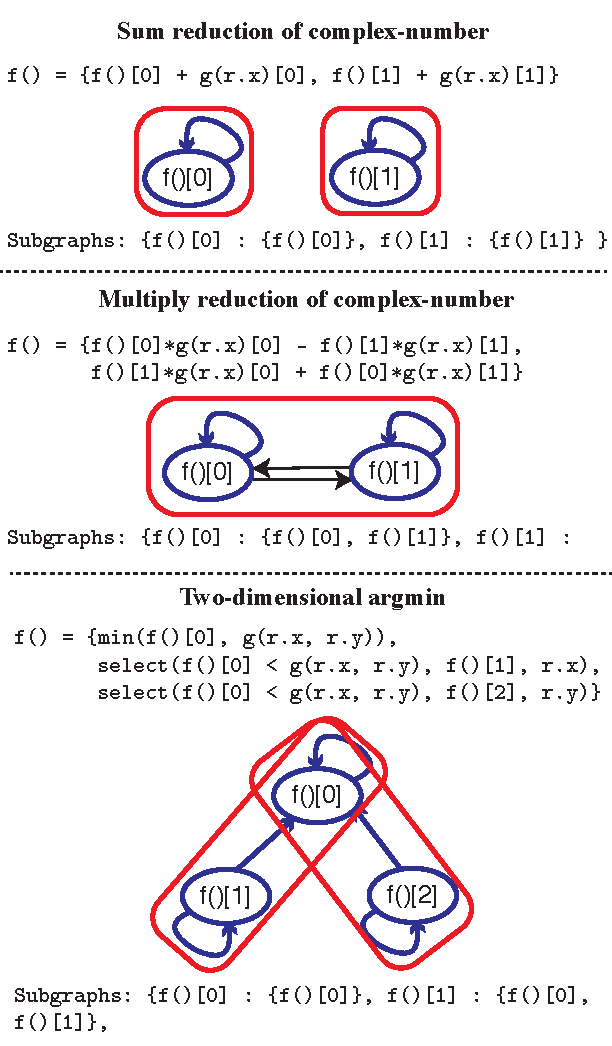
\includegraphics[width=0.5\textwidth]{subgraphs}
\caption{Dependency graphs (in blue) of various Halide $update$ definitions and their subgraph decomposition (each subgraph is marked by a red box).}
\label{fig:subgraphs_decomposition}
\end{figure}

Given a directed dependency graph $G$ of a multi-element tuple reduction, we first decompose $G$ into set of subgraphs for each vertex $V$ in the $G$. After the set of subgraphs are generated, we pre-filter the subgraphs: subgraphs that are fully contained in another subgraph are removed from the set. For the two-dimensional argmin example given above, there are only two relevant subgraphs in the set: the ones originated from \code{f()[1]} and \code{f()[2]}. Since subgraph of \code{f()[0]} is a subset of either subgraph of \code{f()[1]} or subgraph of \code{f()[2]}, it is removed from the set. The problem is then reduced to deducing equivalent binary associative operator and its identity for each of the remaining subgraphs in the set, which in this case is reduced to one-dimensional argmin. 

\begin{proof}
<TODO: Derive formal proof. Why is it okay to decompose the problem into subgraphs and perform the deduction separately?> \\
\end{proof}

After processing each subgraph separately, we need to merge the results. If any of the subgraph is non-associative (or we fail to find the equivalent binary associative operator or an identity), we bail out. If a vertex $x_i$ is in both subgraph $S_{G, p}$ and $S_{G, q}$, we need to ensure that the binary associative operators for that particular tuple element (including their identities) deduced from $S_{G, p}$ and $S_{G, q}$ are consistent. If there is contradiction, we bail out.  

<TODO: update the figure to include the subgraph decomposition>
\begin{figure}
\centering
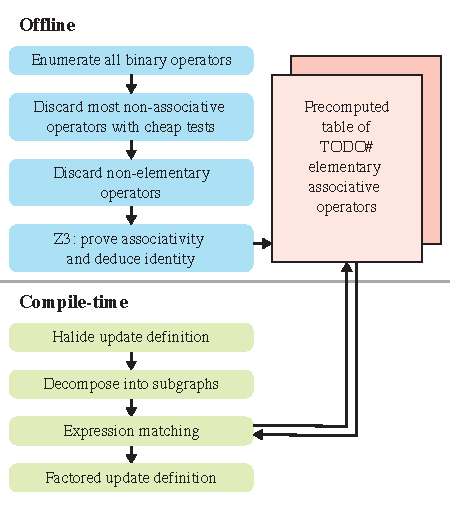
\includegraphics[width=0.5\textwidth]{system}
\caption{To generate the precomputed associative operator table, we synthesize expression tress and use Z3 prover to verify the associativity of an expression tree and to compute its identity. \code{rfactor} takes in Halide \emph{update} definition and the precomputed table to generate the factorized \emph{update} definition. If the directed dependency graph of the \emph{update} is decomposable, \emph{rfactor} reduces the problem into sub-problems which are solved separately and merges those results.}
\label{fig:system} 
\end{figure}
